%
% variation0.tex
%
% (c) 2024 Prof Dr Andreas Müller
%
\begin{figure}
\centering
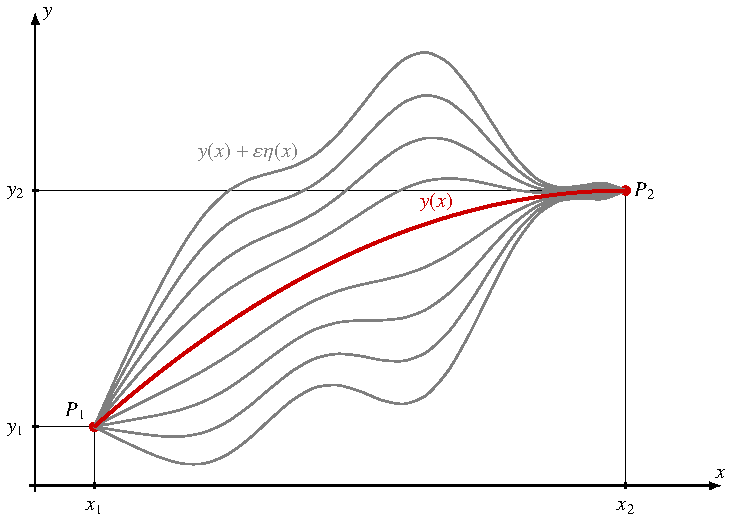
\includegraphics{chapters/020-variation/images/variation0.pdf}
\caption{Variation einer Funktion $y(x)$ durch Addition eines Vielfachen
$\varepsilon\eta(x)$ einer Funktion $\eta(x)$, die in den Endpunkten
des Definitionsintervalls $[x_0,x_1]$ verschwindet: $\eta(x_0)=\eta(x_1)=0$.
\label{buch:variation:fig:variation0}}
\end{figure}
